\section{Synthesis}
The tessellation phase extracts tiles $N\times N$ from each image. Starting from a matrix of grey pixels, represented as a matrix in $\left[0,1\right]^{h \times w}$, where $h$ is the height and $w$ the width of the image.

\noindent Al termine di questa procedura, ogni immagine viene rappresentata come un elenco di tessere, motivo per cui questa fase è chiamata "sintesi": infatti, risulta difficile ricostruire l'immagine originale a partire dalle tessere. Questo processo complica notevolmente qualsiasi tentativo di falsificazione dell'opera, poiché ricostruire manualmente un'immagine con una distribuzione di tessere simile a quella originale è estremamente complicato. Inoltre, la dimensione delle tessere nella rappresentazione è ridotta, ma sufficientemente grande da catturare piccoli automatismi della mano dell'autore, dettagli che sono difficilmente riproducibili in modo volontario.

\begin{algorithm}[ht]
\caption{Algorithm for tile extraction}
\begin{algorithmic}[1]
\Function{TilesExtraction}{$\textnormal{M}, \textnormal{h}, \textnormal{w}$}
    \State declare $v$ as matrix $N \times N$ \Comment{$N$ is size of tiles}
    \State $L \gets \texttt{empty list}$ \Comment{will have $(\textnormal{h} - N + 1)\times(\textnormal{w} - N+1)$ elements}
    \For{$row \gets 0$ to $\textnormal{h} - N$, $col \gets 0$ to $\textnormal{w} - N$}
        \For{$i \gets 1$ to $N$, $j \gets 1$ to $N$}
            \State $v[i][j] \gets \textnormal{M}[row + i][col + j]$
        \EndFor
        \State call \texttt{Append}($L$, $v$)
    \EndFor
\EndFunction
\label{alg:SequentialTilesExtraction}
\end{algorithmic}
\end{algorithm}

\begin{figure}[ht]
    \centering
    \begin{subfigure}{0.4\linewidth}
        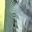
\includegraphics[width=\linewidth]{Figures/example_detail.png}
        \caption{Image detail $32 \times 32$.}
    \end{subfigure}
    \hspace{2cm}
    \begin{subfigure}{0.4\linewidth}
        
\includegraphics[width=\linewidth]{Figures/example_tiles.png}
        \caption{List of tiles $8 \times 8$.}
    \end{subfigure}
    \caption[Illustration of synthesis process]{The synthesis process convert an image in a list of its tiles.}
    \label{fig:puffer_tiles}
\end{figure}
